\documentclass[a4paper]{article}
\usepackage {changepage}
\usepackage{fancyhdr}

\usepackage {fontspec}
\pagestyle{fancy}
\setromanfont{Lantinghei SC Extralight}
\setmonofont{Courier New}
\XeTeXlinebreaklocale ``zh''
\XeTeXlinebreakskip = 0pt plus 1pt
\textheight = 650pt
\begin{document}
\title{实验报告 Lab 2}
\author{姓名:王钦\quad 学号:13349112}
\date{}
\maketitle

\section*{ nslookup}
\hangindent=4em \hangafter=-200{
	1. I use nslookup to find IP of my blog \verb|http://scientist2031.com|\\\\
	{\centering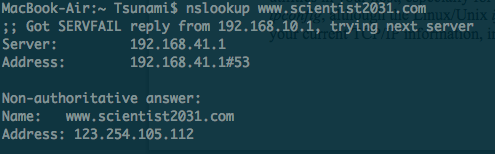
\includegraphics[scale=0.5]{Illustrations/1.png}}\\\\
	2. Because I connect Internet by router,So I use online nslookup to determine the authoritative DNS servers of University of Cambridge.\\
	\verb|Online nslookup:  http://www.kloth.net/services/nslookup.php| \\\\
	{\centering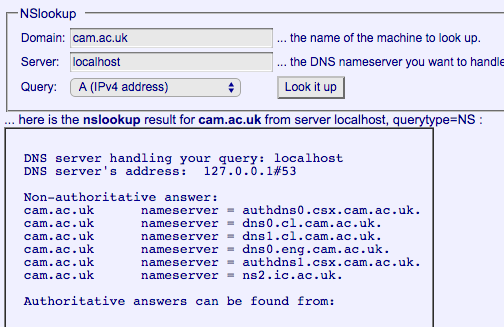
\includegraphics[scale=0.5]{Illustrations/2.png}}\\\\
	3. Because in Question 2,I didn't get the authoritative DNS servers,so I use google DNS \verb|8.8.8.8|\\\\ 
	{\centering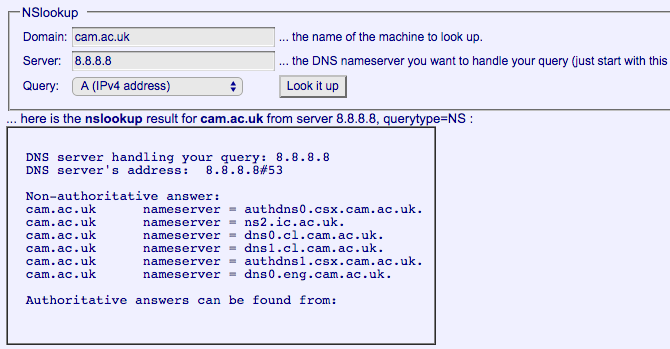
\includegraphics[scale=0.5]{Illustrations/3.png}}\\\\
 }
\section*{ Tracing DNS with wireshark}
\hangindent=4em \hangafter=-200{
	4. They sent over UDP.\\\\
	{\centering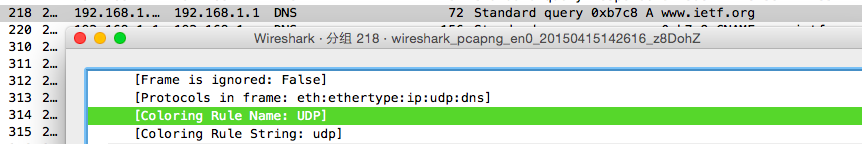
\includegraphics[scale=0.5]{Illustrations/4.png}}\\\\
	5. Destination Port: \verb|55815 (55815)| \ Source Port: \verb|53 (53)|\\\\
	{\centering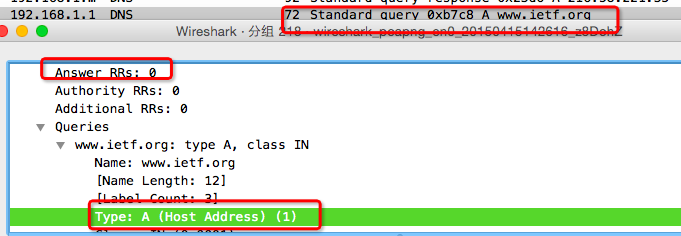
\includegraphics[scale=0.5]{Illustrations/5.png}}\\\\
	6. Yes,They are same IP\\\\
	{\centering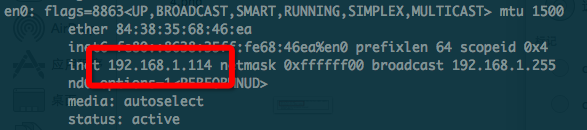
\includegraphics[scale=0.5]{Illustrations/6_1.png}}\\\\
	{\centering
\includegraphics[scale=0.5]{Illustrations/6_2.png}}\\\\
	7. Type: \verb|A (Host Address) (1) |.No,it didn't contain answers\\\\
	{\centering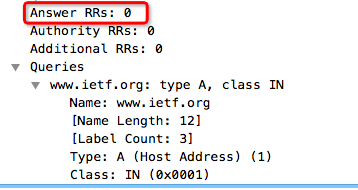
\includegraphics[scale=0.5]{Illustrations/7.png}}\\\\
	8. They are 3 answers provided,Each answers see below\\\\
	{\centering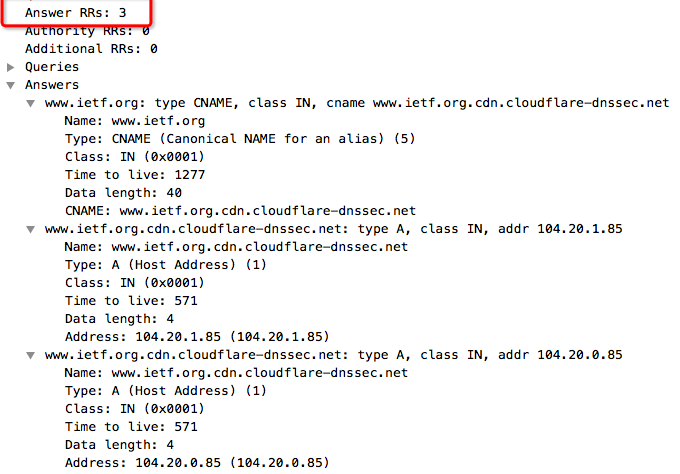
\includegraphics[scale=0.5]{Illustrations/8.png}}\\\\
	9. Subsequent TCP SYN packet sent by my host contain the IP addresses provided in the DNS response message\\\\
	{\centering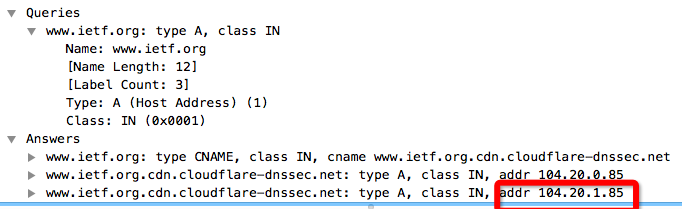
\includegraphics[scale=0.5]{Illustrations/9_1.png}}\\\\
	{\centering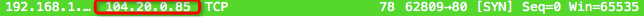
\includegraphics[scale=0.5]{Illustrations/9_2.png}}\\\\
	10. After got the html file,My host doesn't issue new DNS queries\\\\
	{\centering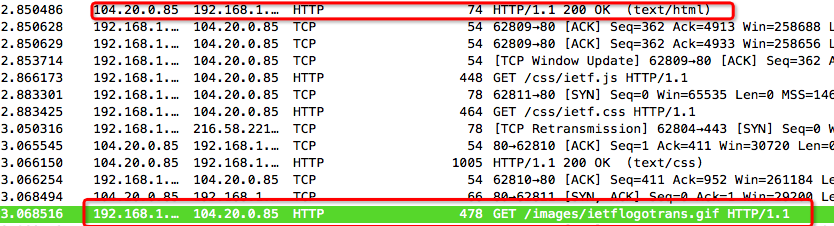
\includegraphics[scale=0.5]{Illustrations/10.png}}\\\\
	11. Destination port for the DNS query message:\verb| 53(53) |,Source port of DNS response message: \verb| 53(53) |.\\\\
	{\centering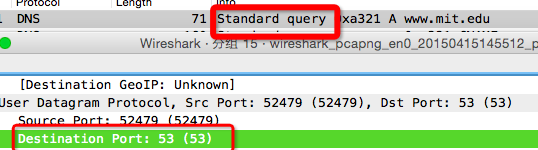
\includegraphics[scale=0.5]{Illustrations/11_1.png}}\\\\
	{\centering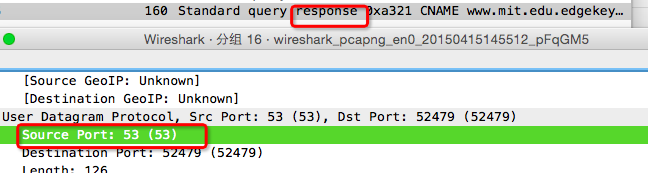
\includegraphics[scale=0.5]{Illustrations/11_2.png}}\\\\
	12. IP address is the DNS query message sent:\verb|192.168.1.1|.No it's my laboratory router ip,my router will send query to real DNS server\\\\
	{\centering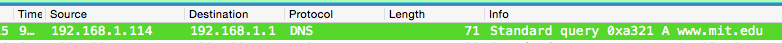
\includegraphics[scale=0.5]{Illustrations/12.png}}\\\\
	13. Type: \verb|A (Host Address) (1) |.Query message didn't contain any answers\\\\
	{\centering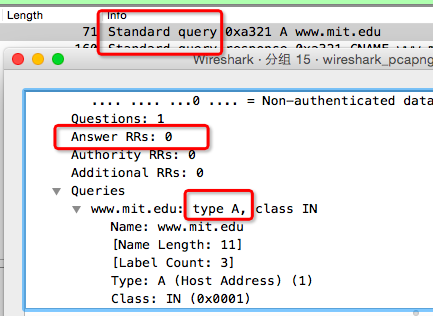
\includegraphics[scale=0.5]{Illustrations/13.png}}\\\\
	14. DNS response message provided 3 answers.The detail of each answers contain see below:\\\\
	{\centering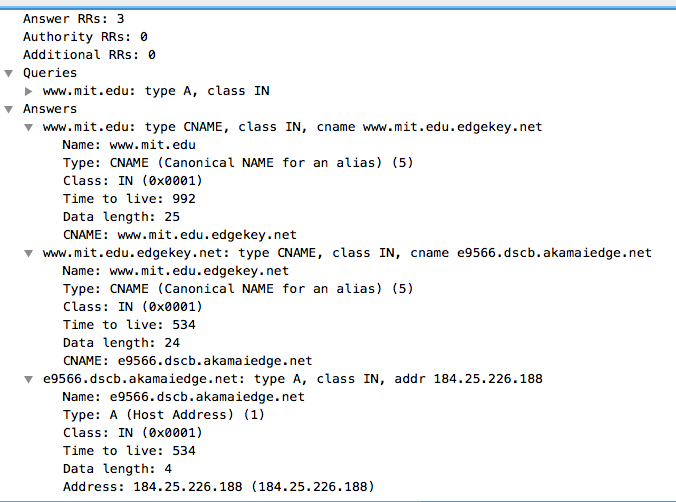
\includegraphics[scale=0.5]{Illustrations/14.png}}\\\\
	15. Sceenshot: \\\\
	{\centering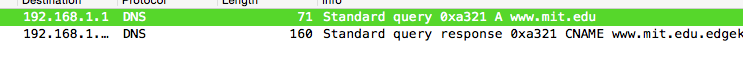
\includegraphics[scale=0.5]{Illustrations/15.png}}\\\\
	16. IP address is the DNS query message sent:\verb|192.168.1.1| ,This address isn't my local dns server,it's my router address.
	My router will send query to real DNS server\\\\
	{\centering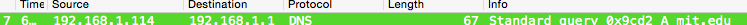
\includegraphics[scale=0.5]{Illustrations/16.png}}\\\\
	17. Type: \verb|A (Host Address) (1)|. Query message didn't contain any answers\\\\
	{\centering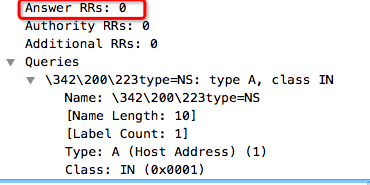
\includegraphics[scale=0.5]{Illustrations/17.png}}\\\\
	18. MIT name servers see below.It doesn't provide IP of the servers.\\\\
	{\centering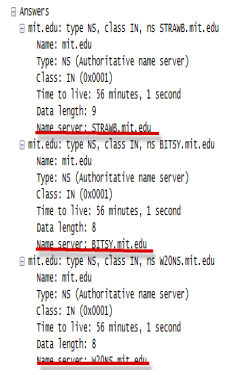
\includegraphics[scale=0.5]{Illustrations/18.png}}\\\\
	19. screenshot.\\\\
	{\centering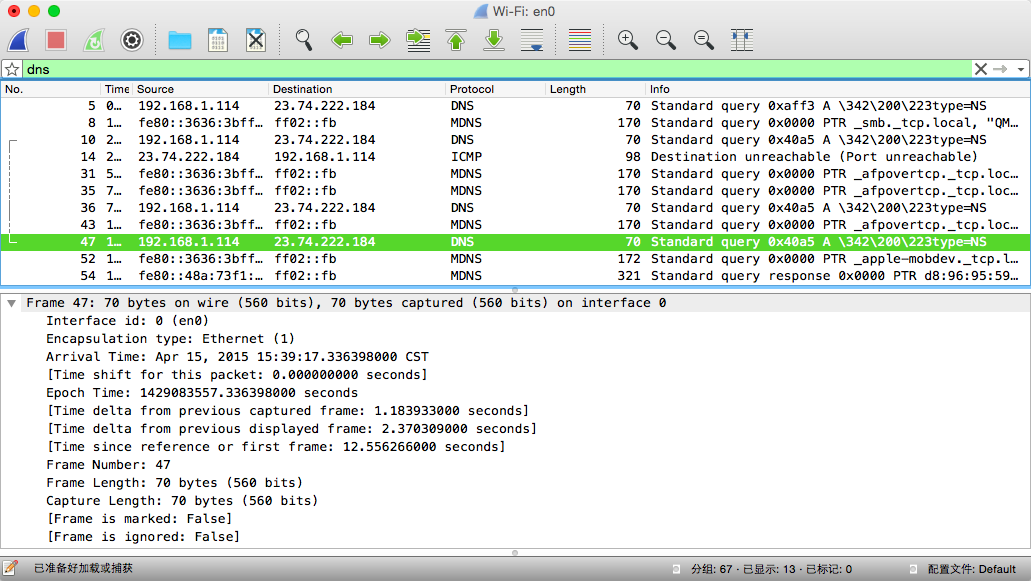
\includegraphics[scale=0.4]{Illustrations/19.png}}\\\\
	20. IP address the DNS query message sent:\verb| Destination: 18.72.0.3 (18.72.0.3)|.This isn't my local DNS server.IP address correspond to bit.mit.edu \\\\
	{\centering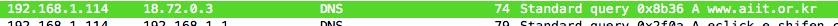
\includegraphics[scale=0.5]{Illustrations/20.png}}\\\\
	21. Type: \verb|A (Host Address) (1)|. Query message didn't contain any answers\\\\
	{\centering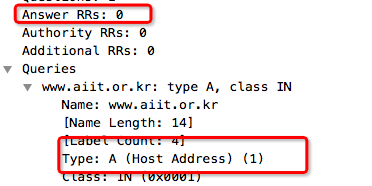
\includegraphics[scale=0.5]{Illustrations/21.png}}\\\\
	22. 3 answers provided.Each of these answers contain see below\\\\
	{\centering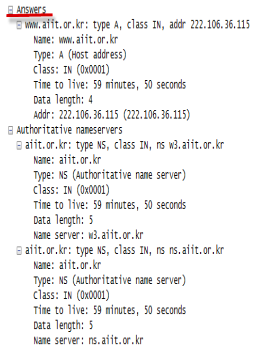
\includegraphics[scale=0.5]{Illustrations/22.png}}\\\\
	23. screenshot.\\\\
	{\centering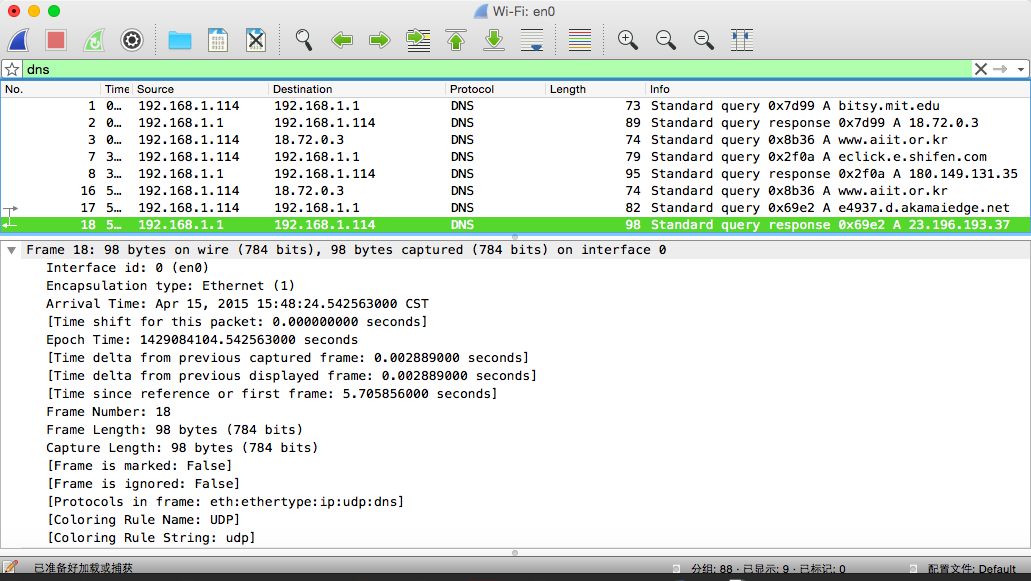
\includegraphics[scale=0.4]{Illustrations/23.png}}\\\\
}

\fancyfoot[OC]{ \footnotesize{https://github.com/wangqin4377/Homework\_Wangqin/tree/master/network/}}
\end{document}


